\subsection{Problem statement}
Our aim is to apply symbolic regression on the output of a simulator. The simulator we use for our experiment is a computationally intensive high performance tool \citep{stride} that models the spread of infectious diseases. 
Epidemiological simulation is a vital tool for policy makers. Simply observing the real world process is a measure of last resort at unacceptable cost in human suffering, and the resulting data is not strictly predictive for new outbreaks. A single outbreak is a sample of a very large configuration space. The focus in policy making lies on prevention and insight, and for these aims simulation and surrogate modelling are essential. A theoretical model cannot approximate within a reasonable error margin the complexity of a real world process, while simulation, with a configurable set of parameters mimicking the real world process, can.
The simulator is configured to model a measles outbreak in a population of 5e5 in the city of Antwerp, Belgium. With immunization for this disease a worldwide concern we would like to obtain a surrogate model that can offer policy makers insights leading to preventative measures. Of vital importance here is the immunization aspect. Our research question for this case is : How does the immunization fraction influence the outbreak of measles?
We investigate this use case within the context of this work, that is, we focus on the convergence characteristics of the process evolving the model rather than the domain specific implications of the surrogate model itself. We are interested in the value of the surrogate model at an intermediary stage in the process. How closely does this model exhibit the same trends as the underlying process? This relation is vital in order to justify our usage of partial results in the feedback loop between practitioner, simulator and regression tool. A single simulation instance is computationally expensive. We would like to construct a surrogate model that approximates the simulator. A surrogate model can offer insights into the underlying process that the resulting data cannot. Symbolic regression offers a white box model in addition to this advantage. We can use symbolic regression to obtain such a model, but in order to do so we need to obtain input and output data.  Generating all simulation output in sequence leads to significant downtime for the practitioner. Using our incremental support detailed we offer the practitioner partial results during this downtime. These results can be used by a domain expert to modify the design of experiment instead of having to wait until the entire process has completed. Our tool is able to reuse the partial results as seeds for new runs. We will investigate if this approach can lead to an improved model.
The value for the practitioner in this approach is twofold : incremental informative results are offered during an otherwise inactive time allowing for a feedback loop with the simulator, and a possible improvement in the final model can be obtained by seeding our regression tool.
\paragraph{Design of experiment}
We would like to have a space filling design that maximizes the sampling of the parameter space while minimizing the number of evaluation points. In this experiment we apply a Latin Hypercube Design (LHD), specifically the Audze-Eglais \citep{AudzeEglais, AudzeEglais2, AudzeEglais3} (AE) LHD which uses the Euclidean distance measure but in addition obtains a uniform distribution of the individual points. 
The AE LHD is based on the concept of minimizing potential energy between design points, a measure based on the inverse of the euclidean distance.
\[
E^{AE} = \sum_{i=0}^{p-1} {\sum_{j=i+1}^{p-1} {\frac{1}{d_{ij}}}}
\]
\paragraph{Simulator configuration}
We construct a DOE with 3 dimensions, 30 points in total using the tool introduced in the work of \citep{DOE}. The following are the parameters used:
\begin{itemize}
\item Basic reproduction number (R0) : the number of persons an infected person will infect, [12-20]
\item Starting set of infected persons (S) : Number of persons in the population that is an infected person at the start of the simulation, [1-500]
\item Immunity fraction (I) : Fraction of the population that is immune to the disease. [0.75, 0.95]
\end{itemize}
The output parameter represents the attack rate, measured as the rate of new cases in the population at risk versus the size of the population at risk. For each parameter we obtain 30 points uniformly chosen in their range. These are then combined in the DOE. The simulator is run once for each configuration. 
\paragraph{Symbolic regression configuration}
We run the experiment with a population size of 20, 30 phases with 60 generations per phase, (10,20,30) datapoints for 3 features, an initial depth of 3 and maximum depth of 6. The 4 best expressions of each phase are archived.
We compare 3 approaches. First we run the CSRM tool on the entire dataset. This is the classical approach, the tool is not seeded and so starts a blind search. In a real world setting this would mean waiting until the simulator has run all 30 configurations.
In our second approach we split the data into incremental sections. After 10 configurations have completed we start the tool on this dataset. The best 4 results are saved to disk, then we run the tool with the result of 20 configurations and use the results from the previous run as a seed. The overlap between the two datasets will influence the effects of the initialization problem. Finally we use the results of the 20-point dataset as a seed for the 30 point run. The cost of running the 10 and 20 point runs to use as seed for the 30 point run is similar to the cost of the 30 point run. To ground the comparison our last approach runs the tool on the data from 30 configurations with double the amount of phases. This means that it has approximately the same number of fitness evaluations as the 10-20-30 combination. We compare all three to see which gains are made and at what cost. We run the experiment distributed to observe the change in convergence characteristics using the seeds of the 10-20-30 combination to combine the distributed and incremental features of our tool.
\subsection{Results}
\subsubsection{Fitness improvement}
We compare both seeded runs and the extended run with the normal 30-point run. In Figure \ref{fig:incrementalgain} we see that the fitness is improved by using the best results of the previous run on a partial data set. We have deliberately split our data set in such a was as to expose a risk here. If we run the tool with 20 datapoints seeded by a run of 10 datapoints, we see that the validated fitness actually decreases compared to a non seeded run. The ratio between new and known data is too large, leading to overfitting. If we seed the best results from the 20-point run into a 30 point configuration we see that both the training and validated fitness values significantly improve. The 30 point run with 60 phases has the same computational cost as the 10-20-30 runs combined, but gains little to nothing in convergence. We see that convergence is slowing, with training fitness improving by a factor of 10 \%, but validation fitness worsens. This is a typical example of overfitting. The combined 10-20-30 run increases validation fitness with a factor of 13\%
\subsubsection{Distributed}
Next we seed a distributed run with the results of the 10/20/30 run and compare the topologies in terms of fitness improvement and speedup. We run the same configuration as before with 25 processes, we use as seeds the 4 best expressions from the 10/20/30 run, and use Tree, Grid, Random and Disconnected topologies. In Figure \ref{fig:usecasedistributed} we compare the gain in fitness on the validation data for the tree, grid and randomstatic topologies compared to the disconnected topology. We can clearly see that the diffusion in the grid topology leads to the highest gain, followed by the tree topology. Interestingly enough, the random topology scored worse than the disconnected topology. This can occur when a local optimum is communicated early to the other processes which then dominates the remainder of the process. The effect on the runtime is measured in Figure \ref{fig:usecasespeedup}. We see that the tree topology has minimal overhead and runs nearly as fast as the disconnected topology where no synchronization or communication overhead is present. The grid topology suffers a 2x performance penalty and the random topology finds the middle ground between the two. During the experiment we observed that the processes in the tree and disconnected topologies varied as much as 4 phases. This is what we expected, in this tree topology the distance between two processes is at most 4 (depth of a 25-node binary tree). This is an important observation, if we increase the number of processes the tree topology will actually scale better. The delay tolerance allows the tree topology this scaling effect.
\begin{figure}
    \begin{subfigure}{0.5\textwidth}
        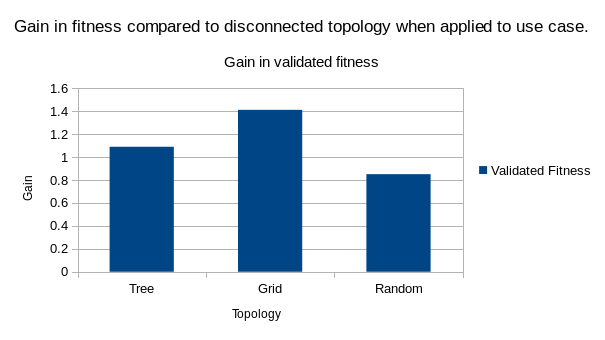
\includegraphics[width=0.8\linewidth]{figures/usecasedistributed.png}
		\caption{Incremental distributed CSRM applied to use case.}
		\label{fig:usecasedistributed}
    \end{subfigure}
    \begin{subfigure}{0.5\textwidth}
        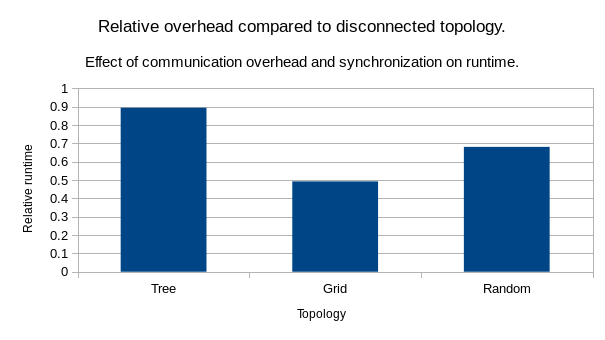
\includegraphics[width=0.8\linewidth]{figures/usecasespeedup.png}
		\caption{Runtime impact of synchronization and communication overhead.}
		\label{fig:usecasespeedup}
    \end{subfigure}
        \begin{subfigure}{0.5\textwidth}
        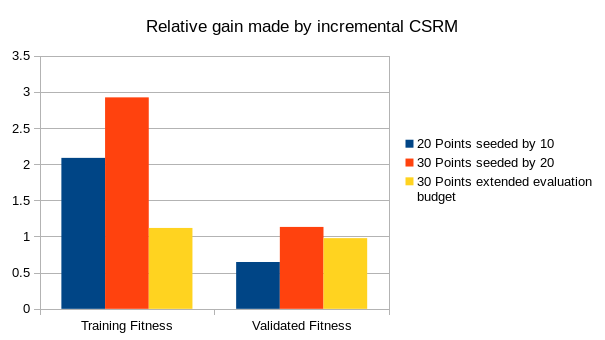
\includegraphics[width=0.8\linewidth]{figures/incrementalgain.png}
        \caption{Incremental fitness gain in CSRM.}
        \label{fig:incrementalgain}
    \end{subfigure}
        \begin{subfigure}{0.5\textwidth}
        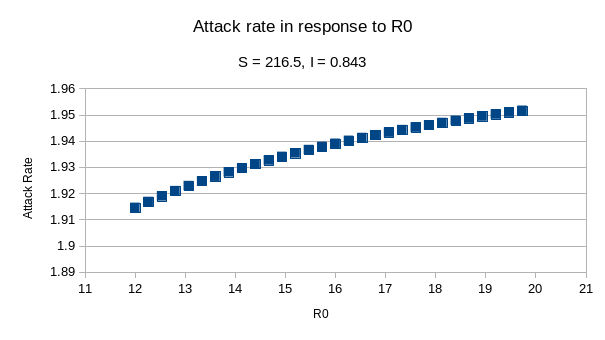
\includegraphics[width=0.5\linewidth]{figures/responseR.png}
        \caption{Response of attack rate to R.}
    \end{subfigure}
    \begin{subfigure}{0.5\textwidth}
        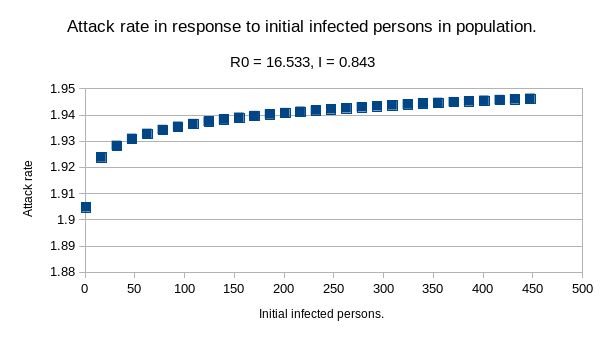
\includegraphics[width=0.5\linewidth]{figures/responseS.png}
        \caption{Response of attack rate to S.}
    \end{subfigure}
        \begin{subfigure}{0.5\textwidth}
        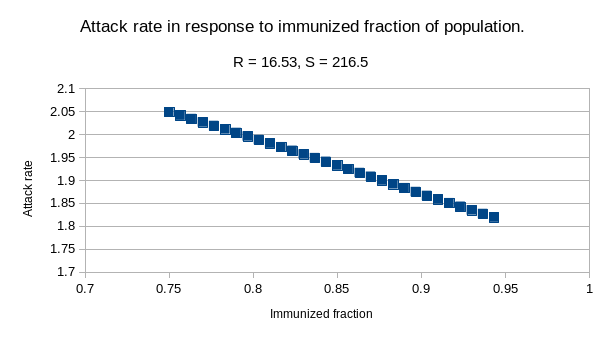
\includegraphics[width=0.5\linewidth]{figures/responseI.png}
        \caption{Response of attack rate to I.}
        \label{fig:usecaseresponseplots}
    \end{subfigure}
    %\caption{Use case : Effect of topology on fitness correlation of distributed processes.}
    %\label{fig:usecasecorrelation}
\end{figure}
We select the best expression returned by the distributed application of CSRM with a tree topology, given its benefits in runtime and scaling. The resulting expression has a fitness value of 0.039 on the full data set. While this value is low, it is still 10 orders of magnitude removed from the optimal. This expression therefore represents an intermediate result and gives us an indication of the value partial results can offer. We use response plots for each parameter in order to isolate the effect each parameter has. We vary each of the parameters while keeping the other two constant. For the constant value we select the midpoint of the range. We then observe the effect on the attack rate. It is important to note that the range of the attack rate is [0,1]. We observe 2 important effects. First, our model produces an attack rate outside of the valid range of [0,1]. There is a scaling factor of 10 between the output of the model and the actual output data from the simulator. This is simply due to the fact that convergence is still in an intermediary phase. An important observation here is that our tool evolves the model based on 30 data points and not the full factorial design. This means that the response plots will use the model to evaluate points that are not necessarily available to our tool to train on. Second, the trend in the response plots is in line with what we expect to see in such a surrogate model. When R0 increases the attack rate increases, which is in line with theoretical and empirical results. A similar trend is visible with the initial number of infected persons, where R0 shows a logarithmic response. Finally, as the immunization fraction increases we see a negative linear response in the attack rate. We have chosen this suboptimal surrogate model to demonstrate that while the exact values of the attack rate are not yet correctly modelled, the expected trends are. This conclusion is vital to justify our incremental approach. We can see that surrogate models will focus on matching the trend first, rather than matching individual points. This is in part due to our usage of the Pearson R correlation coefficent as a basis for the fitness function. 